\usetikzlibrary{positioning}
\section{Project Structure}
The project is divided into several key components:
\begin{itemize}
	\item \textbf{Controllers}: Manage HTTP requests and determine the responses to send back to the client.
	\item \textbf{Services}: Contain the core business logic and handle interactions with external systems such as SSH for executing commands on the robot.
	\item \textbf{Models}: Define the data structures used within the application.
	\item \textbf{ViewModels}: Provide data structures used to pass information between views and controllers.
	\item \textbf{Views}: HTML templates rendered by the controllers to present data to the user.
\end{itemize}
\begin{figure}[H]
	\centering
	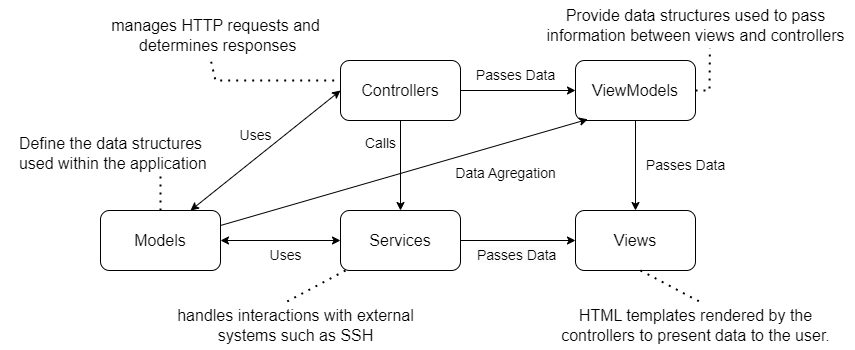
\includegraphics[width=1\textwidth]{Images/ProgramStructure.png}
	\caption{Program Structure}
	\label{}
\end{figure}